\documentclass[dvipsnames]{beamer}

\usepackage{xcolor}
\usepackage{lmodern}
\usepackage{minted}
\usepackage[utf8]{inputenc}
\usepackage{standalone}
\usepackage{tikz}
\usepackage{caption}
\usepackage{adjustbox}
\usepackage{upquote}
\usepackage{hyperref}
\usepackage{multirow}
\usepackage{booktabs}
\usepackage{array}
\usepackage{xspace}
\usetikzlibrary{mindmap,shadows,arrows,positioning,chains,fit,shapes}

\usetheme{metropolis}
\usemintedstyle{manni}

\definecolor{gmitblue}{RGB}{20,134,225}
\definecolor{gmitred}{RGB}{220,20,60}
\definecolor{gmitgrey}{RGB}{67,67,67}

\setbeamercolor{structure}{fg=gmitblue}
\setbeamercolor{frametitle}{fg=white, bg=gmitred}
\setbeamercolor{alerted text}{fg=gmitblue}

\renewcommand\footnoterule{}
\newcommand{\citeurl}[1]{\let\thefootnote\relax\footnotetext{\tiny \textcolor{gmitgrey}{\href{http://#1}{#1}}}}

\begin{document}
  \title{Module Title}
\subtitle{}
\author{ian.mcloughlin@gmit.ie}
\date{}


\begin{frame}
\titlepage
\end{frame}

\begin{frame}
\frametitle{Topics}
\tableofcontents
\end{frame}

\section{About this module}

\begin{frame}{Learning outcomes}
On completion of this module the learner will/should be able to:
  \begin{itemize}
    \item Explain the mathematical and algorithmic underpinnings of 2d and 3d computer graphics.
    \item Apply the basic principles of 2d transformations and animation.
    \item Apply the basic principles of 3d rendering and virtual reality.
  \end{itemize}
\end{frame}

\begin{frame}{Examinations}
  \begin{table}
    \begin{tabular}{p{4cm}r@{\hspace{0.5cm}}p{4cm}}
      Type & \% & Date \\
      \hline
      Continuous Assessment & 50 & Week 6 \\
      End of Semester Exam & 50 & See exams timetable
    \end{tabular}
  \end{table}
\end{frame}

\begin{frame}[fragile]{Code}
  \begin{minted}{html}
<!DOCTYPE html>
<html>
  <head>
    <title>Transformations</title>
    <meta charset="UTF-8">
    <style type="text/css"></style>
  </head>
  <body>
    <script type="text/javascript"></script>
  </body>
</html>
  \end{minted}
\end{frame}


\begin{frame}{Mindmap}
\begin{adjustbox}{max totalsize={.9\textwidth}{.7\textheight},center}
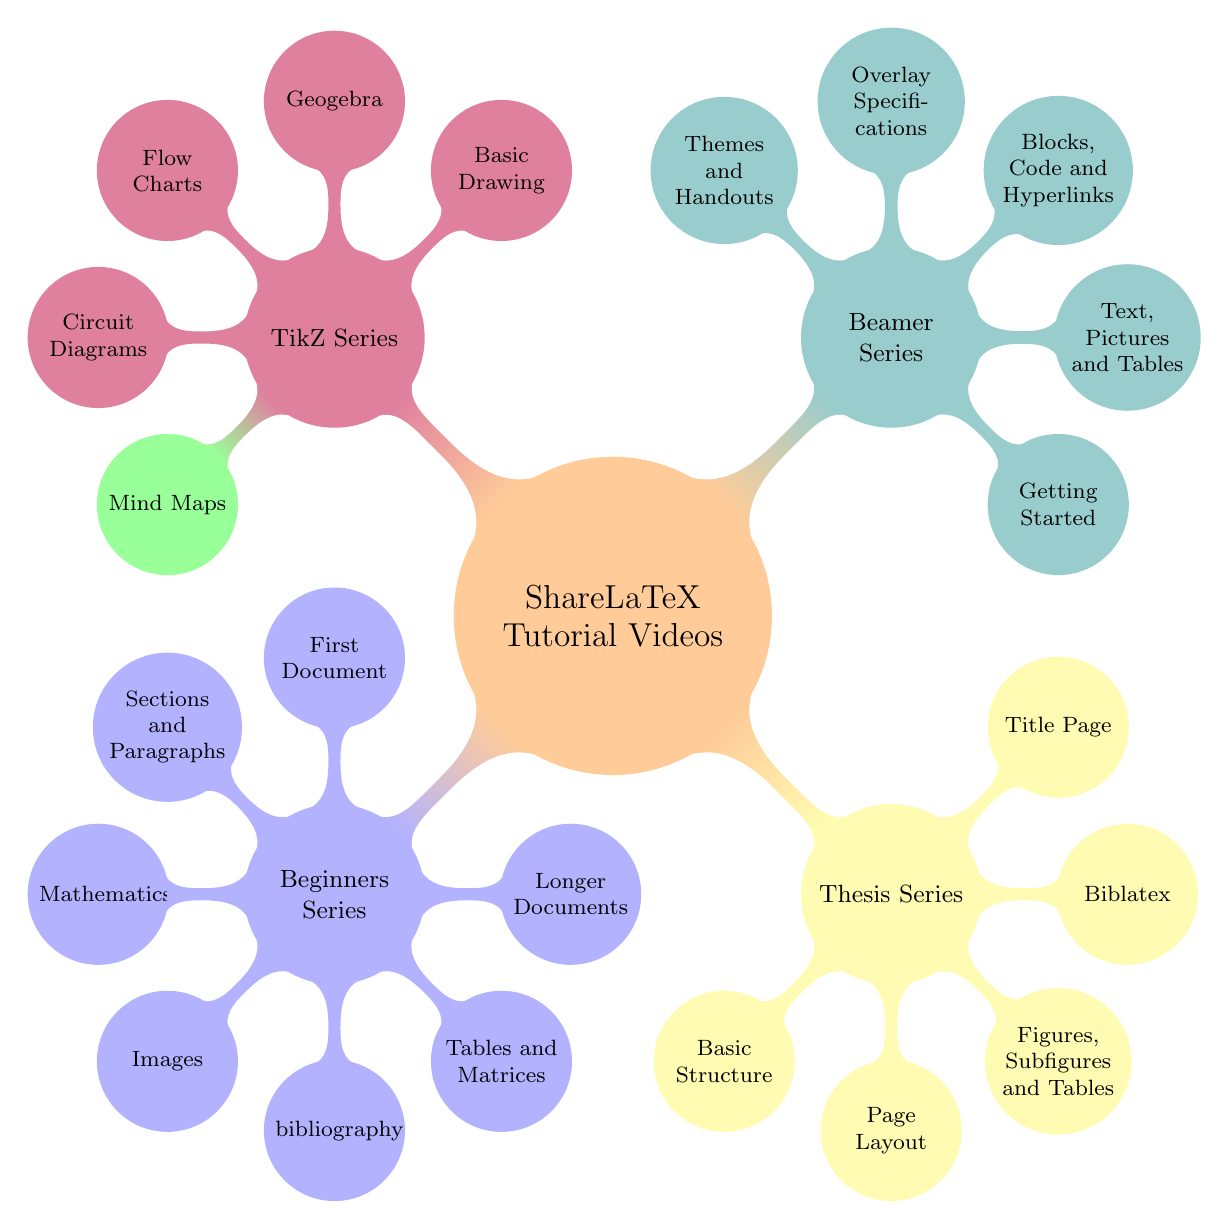
\begin{tikzpicture}[mindmap, grow cyclic, every node/.style=concept, concept color=orange!40,
    level 1/.append style={level distance=5cm,sibling angle=90},
    level 2/.append style={level distance=3cm,sibling angle=45}]

\node{ShareLaTeX Tutorial Videos}
    child [concept color=blue!30] { node {Beginners Series}
        child { node {First Document}}
        child { node {Sections and Paragraphs}}
        child { node {Mathematics}}
        child { node {Images}}
        child { node {bibliography}}
        child { node {Tables and Matrices}}
        child { node {Longer Documents}}
    }
    child [concept color=yellow!30] { node {Thesis Series}
        child { node {Basic Structure}}
        child { node {Page Layout}}
        child { node {Figures, Subfigures and Tables}}
        child { node {Biblatex}}
        child { node {Title Page}}
    }
    child [concept color=teal!40] { node {Beamer Series}
        child { node {Getting Started}}
        child { node {Text, Pictures and Tables}}
        child { node {Blocks, Code and Hyperlinks}}
        child { node {Overlay Specifications}}
        child { node {Themes and Handouts}}
    }
    child [concept color=purple!50] { node {TikZ Series}
        child { node {Basic Drawing}}
        child { node {Geogebra}}
        child { node {Flow Charts}}
        child { node {Circuit Diagrams}}
        child [concept color=green!40] { node {Mind Maps}}
    };
\end{tikzpicture}
\end{adjustbox}
\end{frame}

\begin{frame}{Diagram}
\tikzstyle{decision} = [diamond, draw, fill=blue!20, 
    text width=4.5em, text badly centered, node distance=3cm, inner sep=0pt]
\tikzstyle{block} = [rectangle, draw, fill=blue!20, 
    text width=5em, text centered, rounded corners, minimum height=4em]
\tikzstyle{line} = [draw, -latex']
\tikzstyle{cloud} = [draw, ellipse,fill=red!20, node distance=3cm,
    minimum height=2em]

\begin{adjustbox}{max totalsize={.9\textwidth}{.7\textheight},center} 
\begin{tikzpicture}[node distance = 2cm, auto]
    % Place nodes
    \node [block] (init) {initialize model};
    \node [cloud, left of=init] (expert) {expert};
    \node [cloud, right of=init] (system) {system};
    \node [block, below of=init] (identify) {identify candidate models};
    \node [block, below of=identify] (evaluate) {evaluate candidate models};
    \node [block, left of=evaluate, node distance=3cm] (update) {update model};
    \node [decision, below of=evaluate] (decide) {is best candidate better?};
    \node [block, below of=decide, node distance=3cm] (stop) {stop};
    % Draw edges
    \path [line] (init) -- (identify);
    \path [line] (identify) -- (evaluate);
    \path [line] (evaluate) -- (decide);
    \path [line] (decide) -| node [near start] {yes} (update);
    \path [line] (update) |- (identify);
    \path [line] (decide) -- node {no}(stop);
    \path [line,dashed] (expert) -- (init);
    \path [line,dashed] (system) -- (init);
    \path [line,dashed] (system) |- (evaluate);
\end{tikzpicture}
\end{adjustbox}
\end{frame}

\end{document}